\documentclass[journal,twoside,web]{ieeecolor}
\usepackage{jsen}
\usepackage{cite}
\usepackage{amsmath,amssymb,amsfonts}
\usepackage{algorithmic}
\usepackage{graphicx}
\usepackage{caption}
\usepackage{textcomp}
\usepackage{wrapfig}
\usepackage{anyfontsize}
\usepackage{makecell}
\def\BibTeX{{\rm B\kern-.05em{\sc i\kern-.025em b}\kern-.08em
    T\kern-.1667em\lower.7ex\hbox{E}\kern-.125emX}}
\markboth{}

\begin{document}
\title{Pima Indians Diabetes Dataset}
\author{Athira Bindhu Big Data Analytics and Artificial Intelligence student ID-L00163585
\thanks{Under the supervision of Dr.Shagufta Henna, Letterkenny Institute of Technology}
}

\IEEEtitleabstractindextext{
\begin{abstract}
In this project we are analyze the PIMA Indians diabetes dataset and diabetic prediction is done using different machine learning and ANN analysis.Different machine learning classifier such as support vector machine,XGB Classifier,Random forest classifier,Bernoulli classifier and Gaussian NB is used here and another method ANN is also used here.We are using Apache Spark for filtering and data analysis  along with the Hadoop File System (HDFS).In this project based on the accuracy detection of the different model we are trying to predict the diabetic patients. matplotlib library in python  is used for  visualizing these analyses.
\end{abstract}

\begin{IEEEkeywords}
Machine learning models-SVM,XGBClassifier,Gaussian NB,Bernoulli NB,RandomForestClassifier,pyspark,spark SQL Hadoop,ANN,spark dataframe,one-hot-encoder.
\end{IEEEkeywords}}

\maketitle

\section{Introduction}
\label{sec:introduction}
\IEEEPARstart{D}{iabetes} is actually a lifelong condition caused by the insufficient amount of insulin in our body.And Diabetes means  excessive urination from the body.Insulin is the major component in diabetes and that is made by the pancreas.As the amount of insulin decreases it will lead to diabetes.There are mainly two types of diabetes .Type 1 diabetes  and Type 2 diabetes.Type 1 diabetes arise from childhood or early adult life where as type 2 diabetes is usually develops slowly in adulthood. In our project we are considering with PIMA Indian women having the diabetic condition.\cite{I1}For that we are actually, using there different health related characters and analysed using different machine learning models.PIMA Indians are North American Indian people who are residing in southern Arizona and northern Mexico.We are trying to find out the number of diabetes women from this PIMA Indian group. We are using jupyter notebook interface along pyspark is used for this project.pyspark sql is also used here matplots libraries are used for visualizations and machine learning models are used for classification and prediction of diabetes.Spark is used along with python so that the data classification and prediction is done much faster.Hadoop is also used here.The main aim of this project is identify the number of women having diabetes using machine learning and ANN method.Here we are having three hypotheses
\subsection{Hypotheses}
\begin{enumerate}
    \item To detect diabetes in those women whose age is greater than 25 years and accuracy prediction using machine learning models.
     \item Diabetic prediction using ANN
    \item To find those coming under risk factors using feature engineering.
\end{enumerate}
The other major files and codes regarding this project is uploaded in the github.
(https://github.com/athirabindhu/pima-indians-diabetes.git)

\section{Data description}
\label{sec:data description}
This information was given by the National Institute of Diabetes and Digestive and Kidney Diseases. The purpose of the data set is to use diagnostic metrics in the collection to determine whether a patient has diabetes. Many constraints were imposed on the selection of these examples from a larger database. In this data set we are collecting the details of all pima indian women whose age is greater than 21 years.
This data set is taken from Kaggle\cite{DATA} and  kaggle\cite{data}is used as the source data for this technical project.For this project i have combined the data from the two data set and made it into a single CSV file which is named as "diabetes data".The different fields in our data set is described below.

    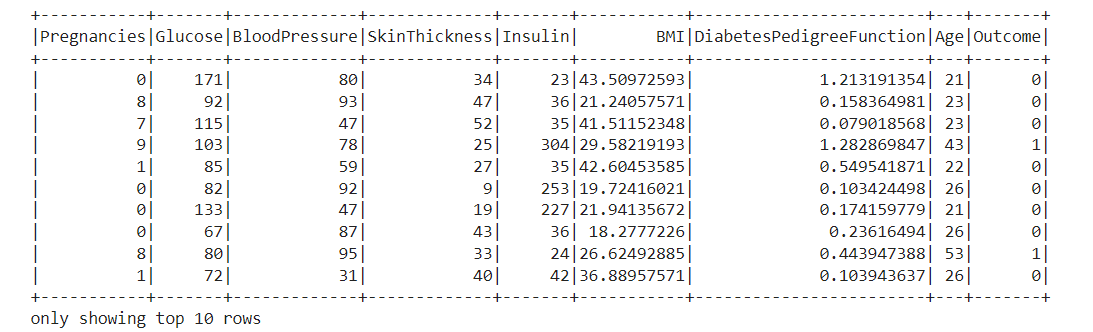
\includegraphics[scale=0.4]{dataset.png}
    \caption{Data set}
    \label{fig1:}
    \centeringfig:-1 Dataset

\begin{enumerate}
    \item Pregnancies:Number of times of pregnancies 
    \item Glucose:Glucose level in blood
    \item BloodPressure
    \item SkinThickness
    \Item Insulin
    \Item BMI:Body mass index
    \item DiabetesPedigreeFunction
    \item Age
    \item Outcome
\end{enumerate}


\section{Related works}
The data set for this project was taken from Kaggle\cite{DATA} and Kaggle\cite{data} and they are merged to form a single CSV file named as diabetes data with wide variety of analysis and visualizations.Most of them are focused in prediction of diabetes and non diabetes people from the data set.In contrast to other contemporary projects, this project  focuses on finding those women who are coming under risk conditions and prediction of diabetes using some popular machine learning models.

\section{Data Aggregation}
Data aggregation is method which is used to collect large amount of data and converting it into a summarized format which can be further used for statistical analysis.In his project we are basically using two data sets and reading as pandas csv file.

\section{Data set Implementation}
This project is implemented in google Colab using Pyspark and required libraries.Visualization and data analysis is done jupyter Notebook using Pyspark.The first step of this data set implementation is done by reading the data in CSV file using pandas.We are importing Apache Pyspark and Hadoop cluster and SQL for this project.After importing the data set we clean our data set and clear all nun value data from our data and make it ready for our data accuracy prediction.
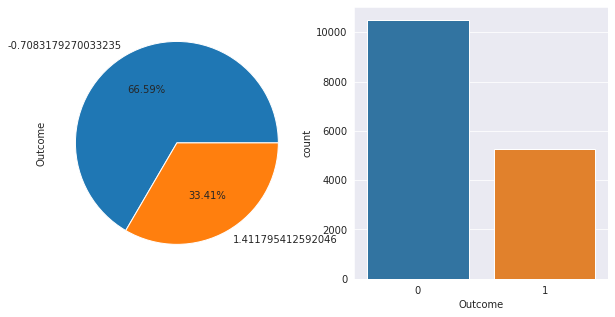
\includegraphics[scale=0.4]{data representation.png}
\caption{fig 2:Data pictorial representation}
\label{fig 2}
fig:-2 Data representation

\subsection{Read the input csv file}
The first step of our project is to read the input data .We collected the data set from Kaggle,and the CSV file format data set is read as spark dataframe by using Pyspark.Spark is a multi-purpose distributed data processing engine which can be used in many situations.Spark is mainly used in big data because it is faster than any other traditional methods this is because spark runs on memory(Random Access memory) which helps to make the processing much faster than on disk drives.Here we are also importing Hadoop.Hadoop is usually used when we are using a large data set which ranges from gigabytes to petabytes.


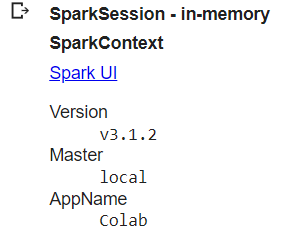
\includegraphics[scale=0.8]{spark.png}
\caption{spark}
\label{fig3-spark}

\section{ Diabetes prediction}

\subsection{Data cleaning}
Our diabetes prediction data set actually containing data's more than fifteen thousand we are mainly creating three goals to solve this data set.After reading the data set we cleaned the data set.The data cleaning is actually a method of cleaning unwanted,wrong,incomplete data or duplicate data from our data set and make our data more neat and clear.When we are trying to merge multiple data sets there arise a high chances of getting duplicated data or multiple data.So to avoid such situation we mainly using data cleaning.
Before data cleaning we need to import some of the important libraries in our python notebook such as Numpy,pandas,matplotlib,datacleaner,seaborn etc.
Through this data cleaning we can remove all unwanted data,missing data,and duplicate data from our data set.

\begin{figure}
    \centering
    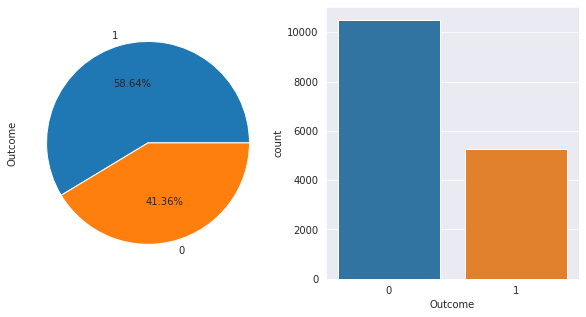
\includegraphics[scale=0.3]{cleaned data.png}
    \caption{Data pictorial representation after cleaning}
    \label{fig 4:}
\end{figure}

\subsection{Read data in SQL}
After cleaning and plotting we can import SQL to read data and  provide certain query to it so that we acquire the desired goals.SQL is the most commonly used programming language for retrieving and organizing data from  relational databases.Database is usually known by a table having rows and columns.The structured query language used in database helps the data set to extract the required data from the specific database for analysis. For attaining a specific information from our database we use queries in sql.This is used because when the data base is very big it is very difficult to sort out data as we need.

\section{Diabetic accuracy prediction using Machine learning models}
We are mainly using five main machine learning models for our diabetic predictions.Basically machine learning models are supervised and unsupervised.There are two types of supervised learning that is classification and regression. Classification involves in predicting class labels and regression involves in predicting numerical values.The five main models used in our project are Support Vector Machine model,XGBClassifier,RandomForestClassifier,BernoulliNB and GaussianNB.
\subsection{Importing libraries}
For predicting the accuracy of the classifiers we had imported some important libraries such as matplotlib,sklearn,standardScaler,accuracy score from sklearn metrics etc.Scikit is the most important machine learning library which can be used in python.Some of the mostly used sklearn toolkit are classification,regression,clustering and dimensionality.
\subsection{Train and Test data}
In machine learning training data set and test data set are two distinct but equally significant components.The training data set is required to teach the machine learning model where as the testing data set is required for training progress and adjusting or optimizing it for better outcomes.Train and test is mainly done in large size data set.Mostly 50 percentage or more than 50 percentage is used for training and remaining data set is used for testing the model.He we use sklearn libraries and importing test and train split to train our data.
\subsection{Accuracy Prediction}
One of our hypotheses is accuracy prediction for the diabetes data set using machine learning models.
The percentage of correct predictions for the test data is known as accuracy. It's simple to figure out simply dividing the number of right guesses by the total number of forecasts.
\subsubsection{Support vector machine models}
Support vector machine is a popular supervised machine learning model which can be used for both classification as well as regression problems.The main goal of svm algorithm is to create a best line or decision that can separate the n-dimensional space into classes.
\subsubsection{XGBClassifier}
XGBoost is a gradient boosting-based ensemble Machine Learning technique that leverages decision trees. The following are some of the ways in which the algorithm distinguishes itself: A wide range of applications are possible: Regression, classification, ranking, and user-defined prediction issues can all be solved using this tool.Here we are using to predict the accuracy of our model.
\subsubsection{RandomForestClassifier}
The Random Forest technique, which is implemented in scikit-learn as the RandomForestRegressor and RandomForestClassifier classes,here we are using RandomForestClassifier  which can be used to determine the relevance of features. The model has a feature importances property that can be used to get the relative importance scores for each input feature once it has been fitted.
\subsubsection{Naive Bayes}
Naive Bayes is supervised machine learning technique.It is a simple classification technique,but has high  functionality.It is basically works on Bayes theorem which gives likelihood of occurrence of the event In this project we are using two naive Bayes learning models such as Gaussian and Bernoulli.Gaussian naive Bayes is very easy to work with because we just need to estimate the standard deviation and mean from the training data.Bernoulli naive Bayes is used for discrete data and works in principle of Bernoulli distribution.

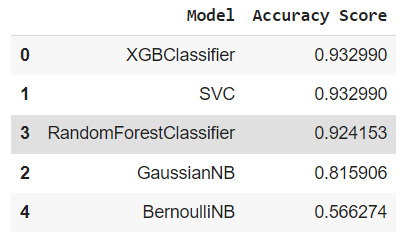
\includegraphics[scale=0.7]{accuracy.png}
\label{fig4}

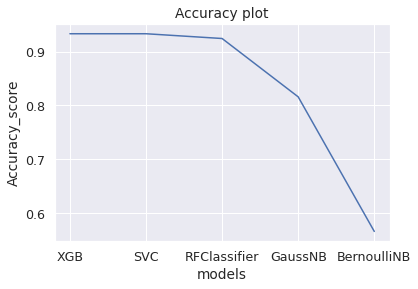
\includegraphics[scale=0.5]{line.png}

The accuracy prediction values in our data set using  different machine learning models are shown in the table above, and these models are sorted in descending order.It is clear from the table that the highest accuracy prediction value is for XGBClassifier and Support vector machine model, both of which have the same value of and the RandomForest Classifier has second highest accuracy value, and Bernoulli NB has the least accuracy.As the value of accuracy and loss is less then it shows that the model makes small errors in most of the data.So for better model the accuracy of the model should be always between 70 and 90 percentage.

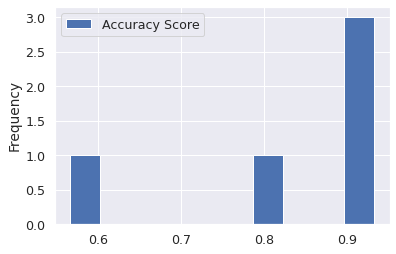
\includegraphics[scale=0.5]{accuracy 1.png}

\section{ANN}
ANN is a type of data processing system .It works in the same way as a human brain does. An ANN is a collection of interconnected processing units that work together to process data. They also produce useful outcomes as a result of it.
The Artificial neural network basically consist of three layers an input layer ,output layer and some hidden layers in between input and output layers.The ANN Units are distributed in two layers: an input layer and an output layer, in the simplest arrangement. Each input layer unit has a single input and a single output that is the same as the input. With a combination function and a transfer function, the output unit connects all of the units from the input layer to its input. There might be several output units. The resultant model is a linear or logistic regression in this scenario. Whether the transfer function is linear or logistic will determine this.In artificial neural network we uses activation function which is a very important part in neural network which determines whether or not a neuron should engaged in the network.

\subsection{Import libraries}
In this technical project for ANN section we are importing libraries such as Numpy,Pandas,matplotlib and keras skompiler,sklearn,train and test.From keras we are importing sequential and dense etc.Keras is a high level deep learning API developed by google for creating neural networks. It is built in Python and is used to make neural network construction simple. It also allows for the calculation of numerous neural networks in the back end.

\subsection{Data Implementation}
First we read our data set "diabetes data" using pd.read csv ,in earlier discussed method we filtered the data and query were generated and accuracy is predicted for only certain group of data(which is women age above 25 years)but here we are predicting accuracy for the entire data set after cleaning it.
The next step for ANN implementation is to create an input layer and output layer and we created only one hidden layer and the activation function we used here is "relu"and"sigmoid".

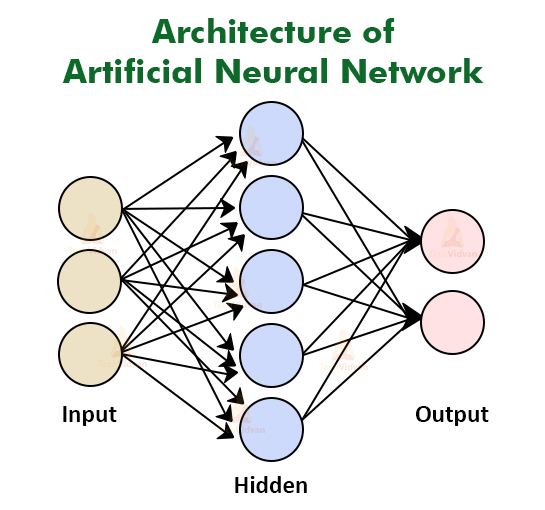
\includegraphics[scale=0.3]{ann.jpg}
\label{fig5}

\subsection{Train and Test data}
The next step was done to train and test the data we have eight independent variables in our data set and we use two-third of data for training and remaining one-third of data for training. An epoch is a measure of unit of time which is used to train a neural network by using all of the training data for a single cycle. Generally We use all of the data just once in era. A pass is done by both forward and backward pass. An epoch is made up of one or more batches in which we train the neural network using a portion of the data set.The epochs value we provided here is 150.

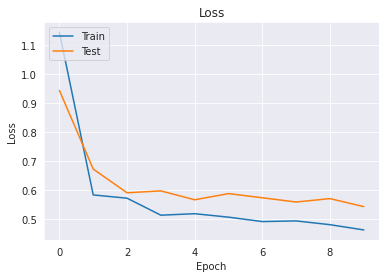
\includegraphics[scale=0.5]{train and test.png}
\subsection{Plot training loss curve}
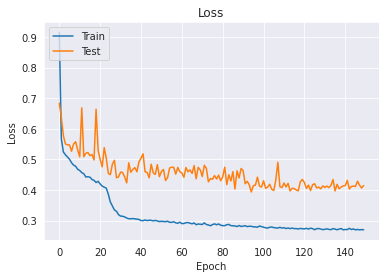
\includegraphics[scale=0.5]{loss.png}

\section{Feature Engineering}
Feature Engineering is the process of extracting data features and translating them into forms that Machine Learning algorithms can understand. The most popular types of data transformation include scaling, discretization, binning, and filling missing data values.Certain factors are more significant than others when it comes to the model's accuracy. It differs from dimensionality reduction in that dimensionality reduction uses existing attributes to combine them, whereas feature selection uses those features to include or exclude them.
Chi-squared test, correlation coefficient scores, LASSO, Ridge regression, and other feature selection approaches are used.

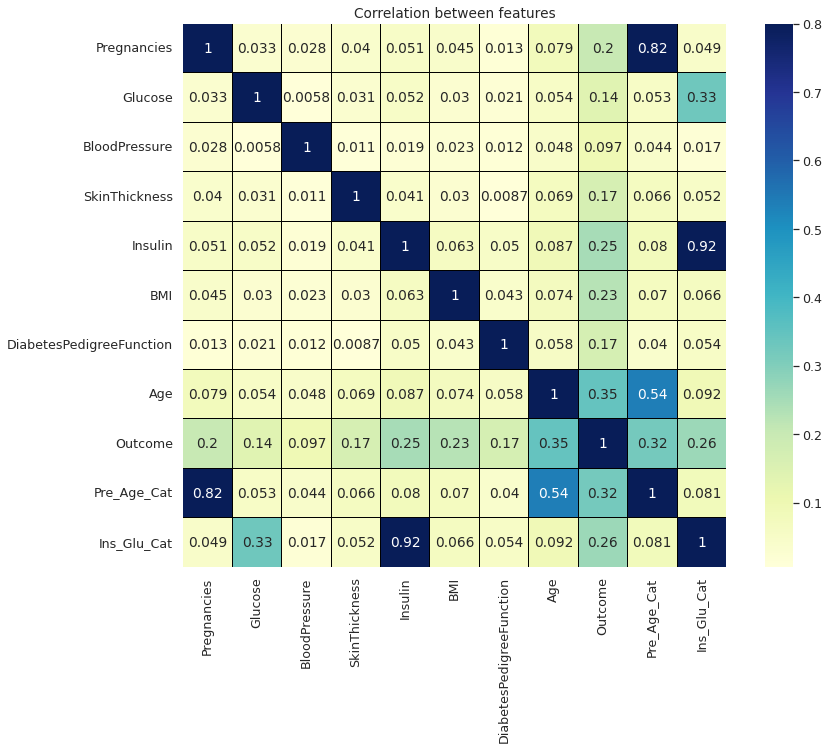
\includegraphics[scale=0.2]{correlation.png}

\subsection{selecting certain features}
Our third hypotheses in this project is to determine those women who are having diabetes and coming under severe risk conditions.For that we selected certain criteria  and imported in the code section and the data is read using pandas and obtained a new data set.
\subsubsection{one hot encoder}
One hot encoding may be defined as the process of changing categorical data variables to be fed into machine and deep learning algorithms,\cite{Alakh Sethi} which improves the model's prediction and classification accuracy.We are also using the label encoders label encoders are basically used to normalize the labels in the given data set.This usually used because it can transform non numerical labels to numerical labels.

\subsection{Feature extraction table plot}
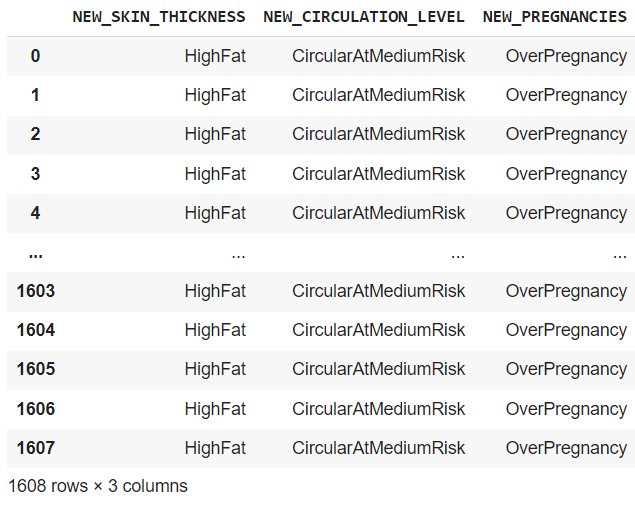
\includegraphics[scale=0.6]{feature extraction.png}

out of 15768 women 1608 women who is having diabetes is coming under severe risk conditions due to various other body conditions also are determined here.

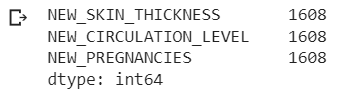
\includegraphics[scale=0.75]{extracted count.png}

\section{Conclusions}
Our project is regarding diabetic prediction in women we have used two data sets from the kaggle\cite{DATA} and we merge that data and uploaded that data as a single csv file named as "diabetes data".This "diabetes data" mainly contains more than fifteen thousand women details.We read the data using pandas and read the data as spark data frame also .In this project we are also using pyspark and sql to read data and to create certain queries.Our main aim in this project was to predict diabetes in women in more efficient way.
As a part of this technical project we used three type of data analysis,the first method is diabetes prediction using five different machine learning approaches,and their accuracy's were measured and plotted.The second hypotheses we were used in this project was artificial neural network,were we included three layer an input layer,output layer and hidden layer and and activation functions are also introduced.The last hypotheses was attained by implementing feature engineering and we was able to find those women who are coming under high risk category.From the data set which is having greater than fifteen thousand we found out 1608 women who are coming under this high risk category.From this data set i was able to understand how different factors in our body leads to various problems,and understood that what all factors can cause diabetes in a women.The study and implementation of this data set was very useful and informative.

\section{Future Work}
This technical project was dealt with determining diabetes affected people from the pima indian's  group.We can use these techniques to sort out a specific group of data from a large group of people in a short span of time.This techniques will have a wide range of applications in many major fields.

\begin{thebibliography}{00}
\bibitem{I1} Andrea Grandi, \emph{Pima Indians diabetes} [Online]. Available: \underline{https://www.andreagrandi.it/2018/04/14/machine-learning-pima-indians-diabetes/}

\bibitem{DATA} kaggle, \emph{kaggle} [Online]. Available: \underline{https://www.kaggle.com/fmendes/diabetes-from-dat263x-lab01}

\bibitem{data} kaggle, \emph{kaggle} [Online]. Available: \underline{https://www.kaggle.com/uciml/pima-indians-diabetes-database}

\bibitem{Alakh Sethi } Alakh Sethi , \emph{Alakh Sethi } [Online]. Available: \underlinehttps://www.analyticsvidhya.com/blog/2020/03/one-hot-encoding-vs-label-encoding-using-scikit-learn/}


\end{thebibliography}


\end{document}
